\documentclass{mnnit}
\usepackage{url}

\begin{document}
\title{Mining Google+ : TF-IDF and Bigram Analysis}
\author{Ishant Sharma 20120001\\* Karan Khanna 20125016\\*  Monalisa Das 20124102\\*  Vikas Saran 20122044 \\* Oindrila Samanta 20124095 \\*}
\supervisor{Dr. Ranvijay}

\specialization{Computer Science \& Engineering}
%\specialization{Computer Science \& Engineering}
\beforepreface
\prefacesection{PREFACE}

\noindent The Google API Console provides a means of registering an application (called a project in the Google API Console) to get OAuth credentials but also
exposes an API key that you can use for “simple API access.” Our Project uses this API key to extract data from Google+ .

\noindent Google+ initially serves as our primary source of data  because it’s inherently social, features content that’s often expressed as longer-form notes that resemble blog entries, and is now an established staple in the social web.

\noindent Our project makes sense of textual information in documents by introducing information retrieval (IR) theory fundamentals such as TF-IDF and collocation detection.

\noindent The analysis on TF-IDF and scoring methods has led us to propose our own implementation of TF-IDF that will consider order of terms in bigram and our own scoring method to rank bigrams.


\prefacesection{ACKNOWLEDGEMENT}
   It is a great pleasure to thank the giants on whose shoulders we stand. First of all, we would like to thank our supervisor Dr. Ranvijay. This project would not have come into being without his kind guidance. He has been a great mentor and the best advisor we could ever have. His advice, encouragement and critique are sources of innovative ideas, inspiration, and causes behind this successful project. The confidence shown by him was the biggest source of inspiration for us. We are highly obliged to all the faculty members of Computer Science and Engineering Department for their support and encouragement. We also thank to our Department Head, Dr. R. S. Yadav for providing excellent facilities and relaxations without which this work was not easy.

\afterpreface

\chapter{INTRODUCTION}
This project presents the details of implementation of finding collocations in documents and applying Term Frequency Inverse Document Frequency to rank documents for each collocation.
Our Thesis basically revolves around the existing implementation of TF-IDF for bigrams and Scoring Methods to Rank Bigrams.
It discusses about the drawbacks in TF-IDF , our modified implementation of TF-IDF and proposal of a scoring method to rank bigrams.
It also discusses about the applications of these in various fields.

 
\newpage

\section{Motivation}
Rapid advances in data collection and storage technology have enabled organizations to accumulate vast amounts of data. However, extracting useful information has proven extremely challenging. Mining is a technology that blends traditional data analysis methods with sophisticated algorithms for processing large volumes of data. It has also opened up exciting opportunities for exploring and analyzing new types of data and for analyzing old types of data in new ways. 



\noindent From startups to the Fortune 500, smart companies are getting on data-driven insight, seizing the opportunities of other technologies.
\vspace{10 mm}

\section{Objective}
The posts here in google+ resemble blog entries. We aim to get relevant reviews of a search query. Additionally we can find out the things which any particular user or other users he may be connected with is talking about . We aim to build an interface that provides user the option to query any person by name or google plus Id , the system will display the N topmost bigrams related to that person.Moreover, the user also has an option of choose one of the selected bigram and find out the posts which contains the bigram. 
	
\noindent We aim to remove the drawbacks in the existing TF-IDF and contribute to bigram scoring methods by proposing a new scoring method. 
	

\newpage


\section{Project Outline}

\vspace{40 mm}


 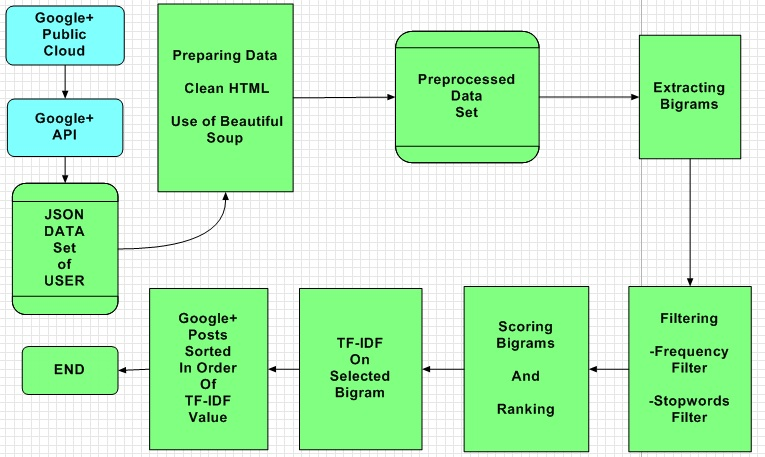
\includegraphics[width=175mm]{Flowchart.jpg}

\chapter{DESCRIPTION}
In this chapter we describe about all the concepts used in this project.

\section{Google+ API }
Anyone with a Gmail account can trivially create a Google+ account and start collaborating
with friends. From standpoint of product, Google+ has evolved rapidly and used some of the most compelling features of existing social network platforms. In Google+ API parlance, social interactions are framed in terms of people, activities, comments, and moments\cite{boole}.

\vspace{2 mm}

\noindent \textbf{People :}
Google+ search API provides the facility to search any user on Google+. Either the username or the Google+ ID stripped out of URL can be used to explore any profile.

\vspace{2 mm}

\noindent \textbf{Activity :}
Activities are the things that people do on Google+.  An activity is essentially a note and can be as long or short as the author likes: it can be as long as a blog post, or it can be devoid of any real textual meaning.

\vspace{2 mm}

\noindent \textbf{Comments :}
Through comments users of Google+ interact with each other. Simple analysis of comments on Google+ would potentially reveal a lot of insights into a person’s social circles or the virality of content.

\section{Introduction of TF -IDF }
TF-IDF, short for Term Frequency–Inverse Document Frequency, is a numerical statistic that is intended to reflect how important a word is to a document in a collection or corpus. It is often used as a weighting factor in information retrieval and text mining. The tf-idf value increases proportionally to the number of times a word appears in the document, but is offset by the frequency of the word in the corpus, which helps to adjust for the fact that some words appear more frequently in general.

\vspace{3 mm}

\noindent \textbf{Term Frequency:}

\noindent A term’s frequency could simply be represented as the number of times it occurs in the text, but it is more commonly the case that you normalize it by taking into account the total number of terms in the text, so that the overall score accounts for document length relative to a term’s frequency.

\vspace{2 mm}

\noindent \textbf{TF(term) = number of occurrences of term in a document / length of document } 

\vspace{2 mm}

\noindent \textbf{Inverse Document Frequency:}
The inverse document frequency is a measure of how much information the word provides, that is, whether the term is common or rare across all documents . In this calculation stop-words are not taken into account. IDF score for a term is the logarithm of a quotient that is defined by the number of documents in the corpus divided by the number of texts in the corpus that contain the term.

         \begin{center}   \textbf{IDF(term) = 1 + Log(N/ M)} \end{center}

\noindent N=Number of documents in overall corpus

\noindent M=Number of documents that contain that term

\noindent A term frequency score is calculated on a per-document basis, an inverse document frequency score is computed on the basis of the entire corpus.

\vspace{2.5 mm}

          \noindent    \textbf{TF-IDF FORMULA  :	TF-IDF = tf * idf }


\noindent To compute the TF-IDF of a Bigram(token1,token2) ,the TF-IDF value of each token is computed and then values of both of them are summed up.
\newpage

\section{Bi-Grams and N-Grams}
Bigrams of a sentence are the two words that appear together in a text/corpus . Similarly n-grams are the n words occurring in a text together in a fixed order\cite{boole}.


\section{Collocations}
A collocation is a sequence of words or terms that co-occur more often than would be expected by chance . We find collocations using collocation finder functionality in NLTK library\cite{boole}.




\section{Scoring Methods}

There are certain methods that are used to give scores to all bigrams and then rank bigrams in order of their importance in the document.
Evaluating and determining the best method to apply in any particular situation is often as much art as science. We discuss here few methods of scoring\cite{nltk1}\cite{nltk2}\cite{nltk3}.

\vspace{1.5 mm}

\noindent \textbf{Raw frequency :}
As its name implies, raw frequency is the ratio expressing the frequency of a particular n-gram divided by the frequency of all n-grams. It is useful for examining the overall frequency of a particular collocation in a text.

\vspace{1.5 mm}


\noindent \textbf{Jaccard Index :}
The Jaccard Index is a ratio that measures the similarity between sets. As applied to collocations, it is defined as the frequency of a particular collocation divided by the total number of collocations that contain at least one term in the collocation of interest. It is useful for determining the likelihood of whether the given terms actually form a collocation, as well as ranking the likelihood of probable collocations. Using notation consistent with previous explanations, this formulation would be mathematically defined as:


                  \[ \frac{freq(term1, term2)}{freq(term1, term2) + freq(\widetilde{term1}, term2) + freq(term1,\widetilde{term2})}           \] 
		

        
        
        
\vspace{1.5 mm}

\noindent \textbf{Dice’s coefficient :}
Dice’s coefficient is extremely similar to the Jaccard Index. The fundamental difference is that it weights agreements among the sets twice as heavily as Jaccard. It is defined mathematically as:

  \[          \frac{2 * freq(term1, term2)}{freq( * , term2) + freq(term1, * )}         
                   \] 
                    
           
            
            
            
               

\noindent Mathematically, it can be shown fairly easily that:

\noindent Dice           =           2 * Jaccard / 1 + Jaccard


\noindent \textbf{Point Mutual Index :}

\noindent An information-theoretic motivated measure for discovering interesting collocations is point-wise mutual information. 
\newline
\noindent Let the total number of words in the document be 1000.Therefore the number of unigrams are 1000 and number of bigrams are (1000-1)=999.
Let the bigram be (token1,token2)
The probability of the unigrams are evaluated.






\[
\textbf{P1} = probability(token1) 	=\frac{frequency  of  token1}{number  of  unigrams} 
	\]				         								     

\[
\textbf{P2} = probability(token2)	=\frac{frequency of token2}{total number of unigrams}	\]						      
	


\[
\textbf{P3} = probability(token1,token2)=\frac{frequency of(token1,token2)}{total number of bigrams} 
		                   				          \]		        
			  			   		    
			  			   		    
			  			   
\[
\textbf{PMI} 	= \frac{P3}{ P1 * P2}   \]         								 
           					
                   						
                   						
                   						
                   						
                   							 


\noindent Since the evaluated value might be large hence we take the log of the evaluated value which is declared as the PMI.

\newpage

\section{Spearman's rank correlation coefficient or Spearman's rho}

Spearman rank correlation is a non-parametric test that is used to measure the degree of association between two variables.  It was developed by Spearman, thus it is called the Spearman rank correlation.  Spearman rank correlation test does not assume any assumptions about the distribution of the data and is the appropriate correlation analysis when the variables are measured on a scale that is at least ordinal.

\noindent The following formula is used to calculate the Spearman rank correlation:
\[
 \rho = {1- \frac {6 \sum d_i^2}{n(n^2 - 1)}}.
\]
Where:
\newline
P= Spearman rank correlation.
\newline
di= the difference between the ranks of corresponding values Xi and Yi.
\newline
n= number of value in each data set.
\vspace{3 mm}
\newline

\noindent In statistics, the value of the correlation coefficient varies between +1 and -1.  When the value of the correlation coefficient lies around ± 1, then it is said to be a perfect degree of association between the two variables.  As the correlation coefficient value goes towards 0,the relationship between the two variables will be weaker.

\newpage 

\chapter{HYPOTHESIS}

\section{Problem Description}
The problem we are trying to solve is that while TF-IDF is a powerful tool that’s easy to use,it has a few important limitations that have been conveniently overlooked :


\begin{enumerate}
\item  It treats a document as a “bag of words,” which means that the order of terms in both the document and the query
itself does not matter.

For example, querying for “Green Mr.” would return the same
results as “Mr. Green” if we didn’t implement logic to take the query term order into
account or interpret the query as a phrase as opposed to a pair of independent terms.
But obviously, the order in which terms appear is very important.
\item Even if one of the unigrams in the Bigram is not present in a post, yet that post will have a positive value of TF-IDF for that bigram.

\item  In performing an n-gram analysis to account for collocations and term ordering,the existing TF-IDF still face the underlying issue that  all tokens with the same text value mean the same thing

\item A homonym is a word that has identical spellings and pronunciations to another word but whose meaning is driven entirely by context, and any homonym of your choice is a counterexample. Homonyms such as book, match, cave, and cool are a few examples that should illustrate the importance of context in determining the meaning of a word.
 
\item String comparisons are case-sensitive, so it’s important to normalize terms so that frequencies can be calculated as accurately as possible. However, blindly normalizing to lowercase can also complicate the situation since the case used in certain words and phrases can be important.
For example-
“Mr. Green” and “Web 2.0” are two examples worth considering. In the case of “Mr.
Green,” maintaining the title case in “Green” could potentially be advantageous
since it could provide a useful clue to a query algorithm that this term is not referring
to an adjective and is likely part of a noun phrase.

\end{enumerate}


\noindent Apart from the above mentioned problems, evaluating the rank of collocations and determining the best scoring method to apply in any particular situation is often as much art as a science.


\section{Proposed Solution }

\textbf{Proposed TF-IDF :}

\noindent In the existing TF-IDF we sum up the individual TF-IDF of the terms.Hence the order of terms is not being preserved.So, in our proposed solution we have considered the bi-gram as a whole. 


\noindent To calculate the TF of Bigram in a particular post/document, the steps are :
\begin{enumerate}
\item The number of occurrence of Bigram in a post is calculated.Let the count be t.
\item The total number of Bigrams in post will be total number of words - 1.Let this count be T1.
\item  The number of bigrams which contains stopwords are removed.Let the count be  T2.
\item The effective total number of bigrams in post = T1 - T2.
    \[TF of the bigram    =     \frac{t}{ T1 - T2}	 \]
     	
				      	       
\end{enumerate}






\noindent To calculate the IDF of Bigram in a particular post/document, the steps are :

\begin{enumerate}
\item Calculate the number of posts in which the Bigram is present.Let the value be L1.
\item Calculate the total number of post, i.e the length of the corpus.Let the value be L2.
\item IDF of the bigram  = 		1 + Log(L1/L2)

\end{enumerate}

\noindent The improved TF-IDF of the Bigram = Improved TF * IDF.

\noindent  proposed method preserves the order of the term.





\vspace{3 mm}

\noindent \textbf{Proposed Scoring Method :}
This method gives more importance to those bigrams  in which the occurring unigrams do not occur with any other bigram. 

\noindent Let the bigram be (token1,token2)

\[
Score  =	\frac{f(token1,token2)}{f(token1)* f( token1, \widetilde{token2})   +  f(token2)* f( \widetilde{token1}, token2 )  +  f(token1,token2)}		\]	    
   
               

\noindent where 


\noindent f( token1,token2 ) 	         =  frequency of the bigram


\noindent f( token1 )	     	         =  frequency of the unigram token1


\noindent f( token2 )	     	         =  frequency of the unigram token2


\noindent f(token1, $\widetilde{token2}$)	     =  frequency of  bigrams in which  token1  appears  without  token2


\noindent f($\widetilde{token1}$, token2)	     =  frequency  of   bigrams in  which  token2  appears  without  token1



\noindent \textbf{Steps:}
\begin{enumerate}
\item Calculate the bigram frequency f(token1,token2)  and the the frequency of unigrams occurring in that bigram , i.e , f(token1)  and f(token2).
\item To find number of occurrences of token1 as a bigram with any other token except token2 , i.e, f(token1, $\widetilde{token2}$) = f(token1) - f(token1,token2).

\item Similarly we evaluate f($\widetilde{token1}$,token2).
\end{enumerate}



\section{Working of Interface Implementing proposed method }

\noindent \textbf{INPUT :}

\begin{enumerate}
\item The Google+ ID or the Google+ Username.
\item Maximum number of collocations required.
\item Number of topmost posts of interest.
\end{enumerate}
 

\noindent \textbf{OUTPUT :}
\begin{enumerate}
\item Required collocations.
\item Topmost posts for selected collocation.
\end{enumerate}




\noindent \textbf{STEPS :}

\begin{enumerate}
\item Click  the “Google+” label to enter the Google+ ID or the Google+ Username.
\item Enter the corresponding detail and Submit.
\item Now click on the “Result G+” option to get the list of the users related to the query.
\item Select the desired Userid to mine.
\item Click on “Mine this User” to let the system collect the required data.
\item Click on “Collocations” to enter the number of collocations required.
\item Submit the number to get the desired collocations.
\item Click on “List of Bigrams” to get the bigrams ranked on the basis of scoring method.
\item Select the Bigram for which the corresponding posts need to be extracted.
\item The corresponding posts will be obtained.
\end{enumerate}



\section{Applications Of Proposed Method}

\noindent The Modified TF-IDF as proposed by us can be used in :

\begin{enumerate}
\item Categorization applications to texts written in programming languages. Applying bigrams in this setup would lead to a
significant success\cite{ron}.

\item Feature wise Product Ranking from Reviews.
\end{enumerate}




\noindent Implementation of Programming Language Classifier :

\vspace{1.5 mm}
\noindent \textbf{Training data} \newline
Set of files of each programming language

\vspace{2 mm}

\noindent \textbf{Testing data} \newline
Source code file to be classified.

\vspace{2 mm}

\noindent \textbf{Output} \newline
Type of Source code file.

\vspace{2 mm}

\noindent \textbf{Steps:}
	\begin{enumerate}
	\item  Build a python dictionary by traversing the training data keeping bigrams as key and the language to which it belongs as value.
	\item Those Bigrams that occur in more than one language data set are discarded.
	\item Traverse the testing code file and find out the bigrams in it.
	\item The result is the language that has the maximum number of bigrams matched with the bigrams of the testing data.
	\end{enumerate}









\chapter{CONCLUSION AND FUTURE WORK}
\textbf{TF-IDF:}\newline
Since we have considered bigram itself while calculating the TF-IDF instead of unigrams , the TF-IDF value will be zero for posts that has a unigram but no relevant bigram. The query "Mr. Green" and "Green Mr." will be treated differently as order of terms in considered.
\newline
\noindent \textbf{The Complexity of the proposed method is O(N),} \newline where N= Total Corpus length.


\noindent \textbf{Scoring Method Comparison with Existing Methods:}
\begin{enumerate}\bfseries
\item Spearman correalaton coefficient with jaccard and dice is 0.796020318207
\item Spearman correalaton coefficient with pmi is 0.736470775601
\end{enumerate}

\noindent This project has a lot of future prospects. The TF-IDF can be further optimized to consider contextual meaning and case sensitivity
by applying advanced parsing with NLP.


\chapter{SNAPSHOTS}
\vspace{10 mm}
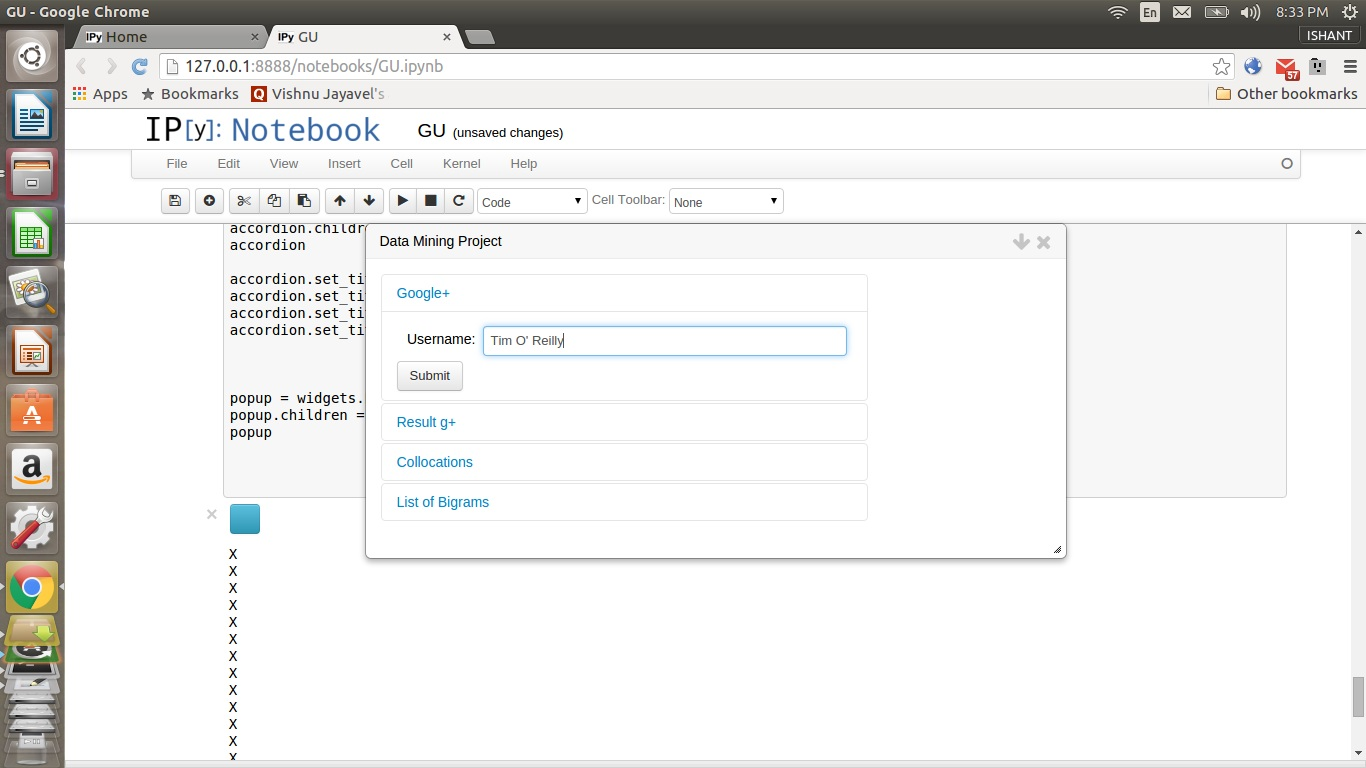
\includegraphics[width=175mm,height=115mm]{Screenshot1.jpg}

\vspace{2 mm}
\begin{center}
\cite{ipythoninfo1}
\cite{ipythoninfo2}
\end{center}

\vspace{120 mm}

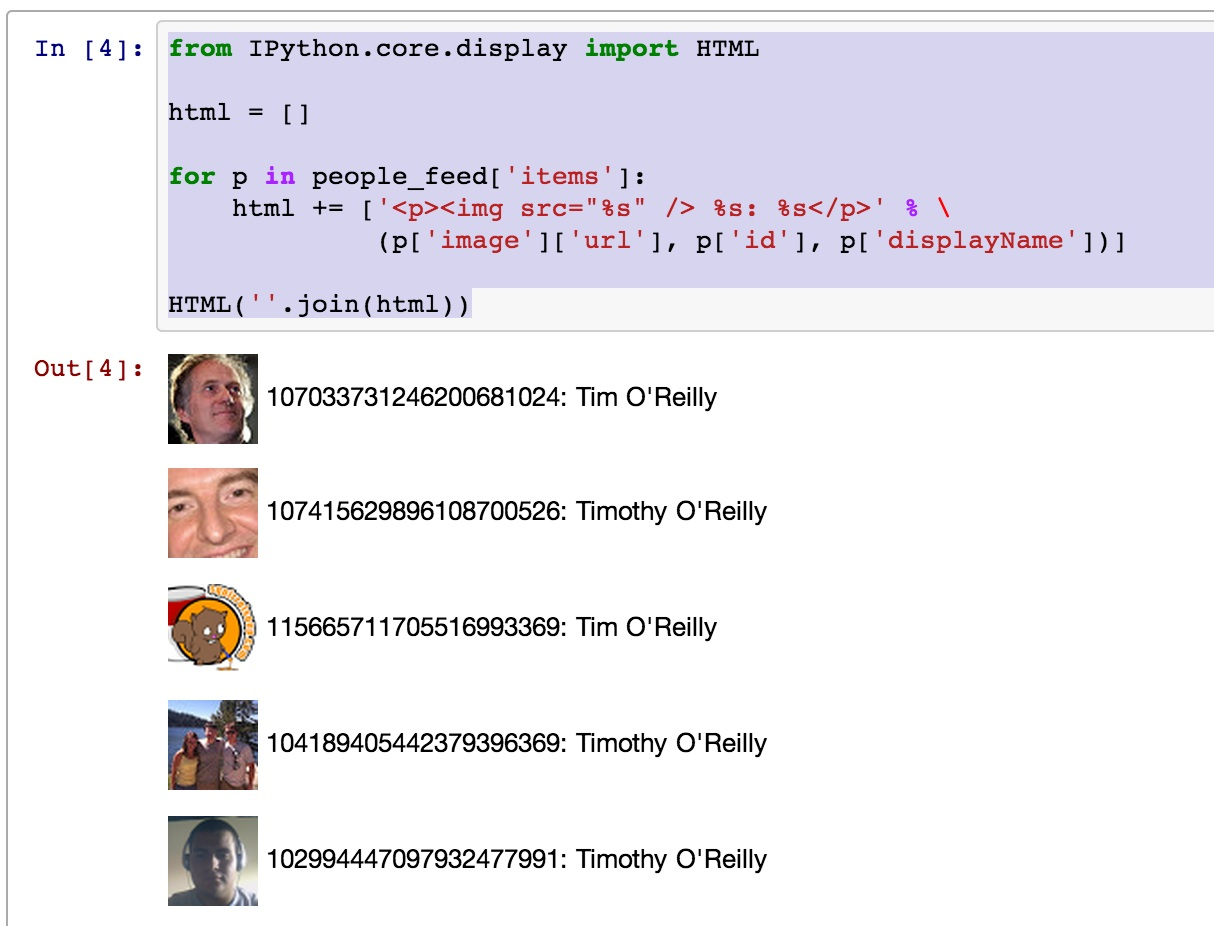
\includegraphics[width=175mm,height=140mm]{Screenshot3.jpg}
\vspace{2 mm}
\begin{center}
\cite{boole}
\end{center}

\vspace{120 mm}


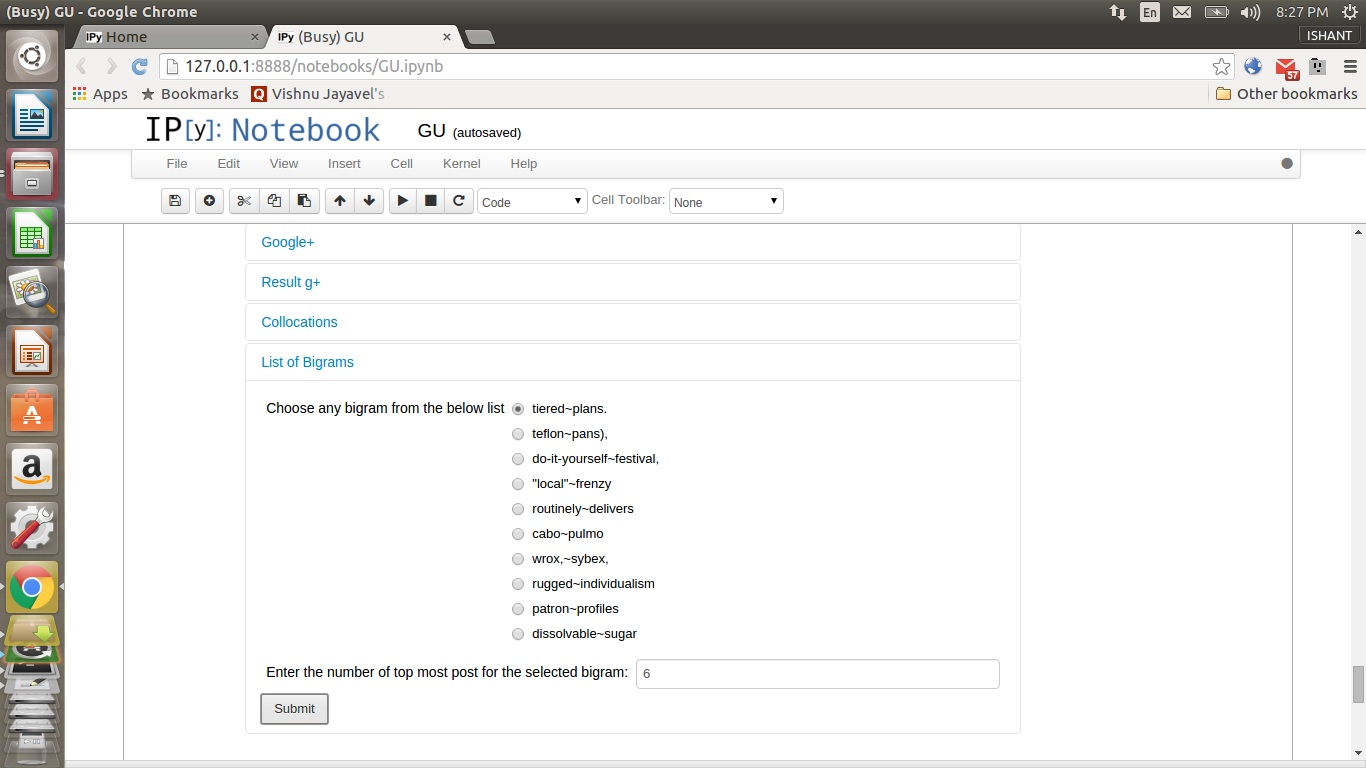
\includegraphics[width=175mm,height=120mm]{Screenshot2.jpg}

\vspace{2 mm}
\begin{center}
\cite{ipythoninfo1}
\cite{ipythoninfo2}
\end{center}

\bibliographystyle{acm}

\bibliography{references}
\cite{boole}
\cite{ron}
\cite{nltk1}
\cite{nltk2}
\cite{nltk3}
\cite{ipythoninfo1}
\cite{ipythoninfo2}


\end{document}
